When you're developing your program---exploring ideas---you'll often find that things get long and out-of-hand. This chapter will help you see both how to handle multiple inputs and multiple outputs, as well as how to reorganize your code to make it more readable.

\section{The Challenge}

You want to develop a circuit that has multiple inputs and multiple outputs. In our case, we'll use pushbuttons as our inputs and and LEDs as our outputs---but the principles we're going to explore will be the same regardless of what serves as the source for your input and the destination for your output.

We know that one button and LED yields a process network with two {\PROCedure}s. This will serve as our starting point.

\vspace{3mm}
\begin{figure}[ht]
  \begin{center}
    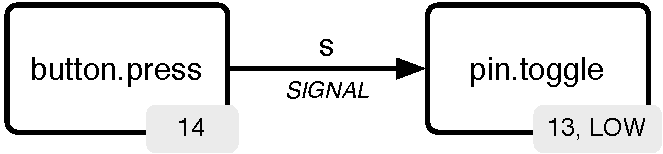
\includegraphics[width=0.8\linewidth]{images/ch4-button-toggle-led}
    \caption{The network from Chapter~\ref{ch4} again.}
    \label{diagram:ch6-button-toggle-led}
  \end{center}
\end{figure}


\section{The Circuit}

This circuit builds on the circuit from Chapter~\ref{ch4}. We add another button (to pin {\constant 3}) and another LED (to pin {\constant 6}).

\begin{figure}[ht]
  \begin{center}
    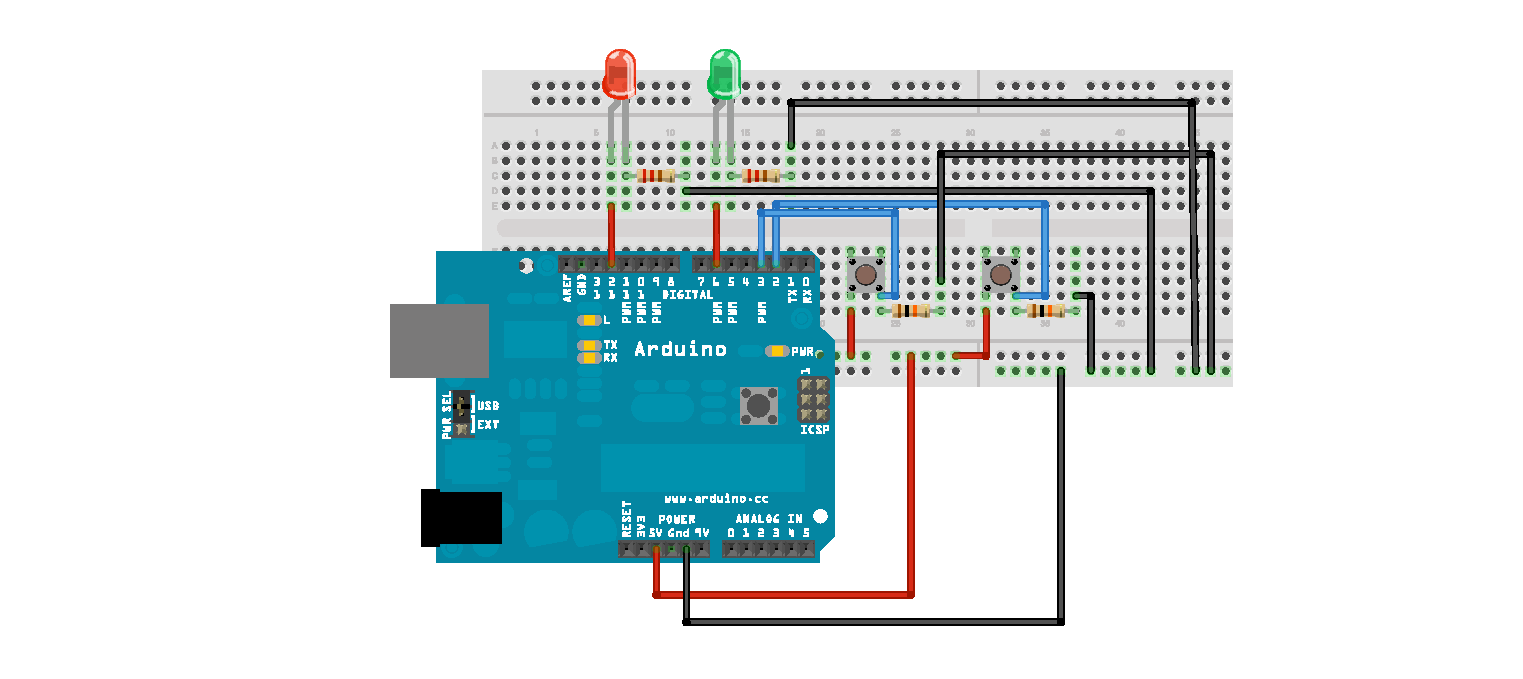
\includegraphics[width=0.8\linewidth]{images/ch6-two-button-circuit}
    \caption{Two buttons, two LEDs.}
    \label{diagram:ch6-two-button-circuit}
  \end{center}
\end{figure}

\newpage

Looking at the process network on ~\vref{diagram:ch6-button-toggle-led}, we can see that it will work just fine with this circuit. That is, we can run the code from the previous chapters and still control one of the LEDs. It we want to handle the other button and LED, however, we'll need another \bp procedures and more \tp procedures.

\section{Reusing Procedures}
Here is the code from Chapter~\ref{ch4}.

\vspace{3mm}
\begin{lstlisting}
PROC main ()
  CHAN SIGNAL s:
  PAR
    button.press(2, s!)
    pin.toggle(13, LOW, s?)
:
\end{lstlisting}

We have one channel {\code s} connecting our button input from pin {\constant 2} to our toggle process controlling the LED on pin {\constant 13}. As it happens, we're able to use {\PROCedure}s more than once, providing them with different parameters. In a picture, the process network looks like Figure~\vref{diagram:ch6-process-network}. 

Put simply, we run the same \PROCedure multiple times, but we provide it will different parameters. One \bp is told to watch pin \pintwo, while the second \bp is told to watch \pinthree. Note, though, that each \CHANnel must have its own unique name. Although it isn't very creative, I've named one channel {\code s1} and the other {\code s2}. 

\newpage

\begin{figure}[ht]
  \begin{center}
    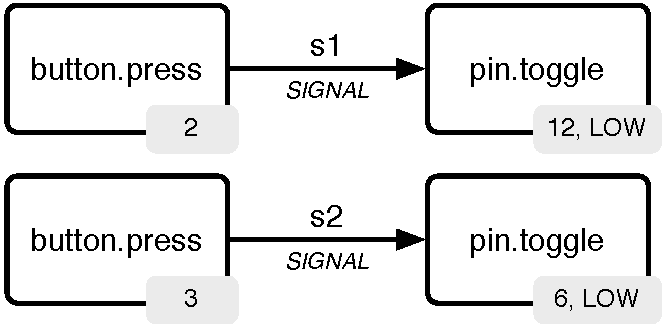
\includegraphics[width=0.8\linewidth]{images/ch6-process-network}
    \caption{Change the parameters to reuse {\PROCedure}s}
    \label{diagram:ch6-process-network}
  \end{center}
\end{figure}

The reason we like using \occam for writing this kind of program is that it is remarkably easy to convert this process network into code. We take the code we wrote before, and we simply run two more processes under the same \PAR. We will have to add one more channel declaration, but that's not so hard. When we're done adding in two more processes, we end up with code that looks like this:

\vspace{6mm}
\begin{lstlisting}
PROC main ()
  CHAN SIGNAL s1, s2:
  PAR
    button.press(2, s1!)
    pin.toggle(13, LOW, s1?)
    button.press(3, s2!)
    pin.toggle(6, LOW, s2?)

:
\end{lstlisting}

\newpage

\section{Managing complexity}
When programming in \occam, we like the fact that we can add more {\PROCedure}s underneath a \PAR and handle more things concurrently (``at the same time''). Unfortunately, our \PAR can grow a bit unwieldy. Eventually, it's nice to be able to bundle things up and shrink the amount of code we have in any one \PROC. If you prefer, we're going to reverse the process we saw in the last chapter: instead of breaking one process apart, we're going to build a new one by putting smaller pieces toether.

For example, it might be nice to introduce a new \PROC called {\code b2p} (short for ``button to pin''). This \PROCedure will take two parameters: the pin that a button is connected to ({\code b.pin}), and the pin that an LED is connected to ({\code l.pin}). It will ``hide'' from us the fact that there is a channel communication between \bp and \tp. 
 
We might start our code this way:

\vspace{3mm}
\begin{lstlisting}
PROC b2p (VAL INT b.pin, l.pin)
:
\end{lstlisting}

The two parameters that this \PROCedure is going to expect are {\strong constants}, or numbers that cannot be changed. In \occam, we can't say {\code CONSTANT}, but we can say {\code VAL INT}, which means it is a number (an \INTeger) and it is a \VALue, not a variable. 

\newpage

Inside of this \PROC, we can build a small process network. Specifically, we'll put \bp and \tp, and connect them up as we did before.

\vspace{3mm}
\begin{lstlisting}
PROC b2p (VAL INT b.pin, l.pin)
  CHAN SIGNAL s:
  PAR
    button.press(b.pin, s!)
    pin.toggle(l.pin, LOW, s?)
:
\end{lstlisting}

The critical change made in connecting \bp to \tp  is that we substituted {\code b.pin} for one of the parameters of \bp, and {\code l.pin} for one of the parameters of \tp. 

Now that we have combined \bp and \tp in one \PROC called {\code b2p}, we can use that in the rest of our code. We can now write our {\code main} \PROC this way:

\vspace{3mm}
\begin{lstlisting}
PROC main ()
  PAR
    b2p(2, 12)
    b2p(3, 6)
:
\end{lstlisting}

If we were to ``peel back'' both of these {\PROCedure}s, we'd end up right back where we started: with two copies of the \bp ~\PROC and two copies of \tp, each connected by their own channel. This way, we've simplified our program, and we can now reuse {\code b2p}, our new \PROC, as part of other process networks.

\newpage

\section{The Code}

Here is the full program from this chapter, in one place.

\vspace{3mm}
\begin{lstlisting}
PROC b2p (VAL INT b.pin, l.pin)
  CHAN SIGNAL s:
  PAR
    button.press(b.pin, s!)
    pin.toggle(l.pin, LOW, s?)
:

PROC main ()
  PAR
    b2p(2, 12)
    b2p(3, 6)
:
\end{lstlisting}

\section{Breakage}
As always, there are many ways to break your code. Breaking code is part of how you learn.

\begin{description}
	\item[Bad constants]\ \\
	What happens if you use a value for a pin that is too large (eg. {\constant 42})?
	\item[Forget the {\keyword VAL}]\ \\
	What happens if, in your definition for {\code b2p}, you forget the word {\keyword VAL}?
	\item[Reuse some pins]\ \\
	What happens if you try and use {\code b2p} twice, but you use the same constants both times?
	\item[Mixup pins]\ \\
	What happens if you mix up {\code b.pin} and {\code l.pin} in the \PROC {\code b2p}?
	\item[Switch the order]\ \\
	Does anything break if you put one {\code b2p} before the other in the \PAR?
	\item[Forget a comma]\ \\
	There are several place that we've used commas. What happens if you leave one out?
	\item[Use a channel twice]\ \\
	If you go back to the code from the middle of the chapter, what happens if you use {\code s1?} more than once? What happens if you use {\code s2!} more than once?
	\item[Fail to use a channel]\ \\
	What happens if you declare a channel but never use it? Add \\
	\ \\
	{\code CHAN SIGNAL oops:} \\
	\ \\
	before the \PAR in your {\code main} and see what happens.
\end{description}
